%----------------------------------------------------------------------------------------
%    PACKAGES AND THEMES
%----------------------------------------------------------------------------------------

\documentclass[aspectratio=169,xcolor=dvipsnames]{beamer}
\setbeameroption{show notes} %TODO: Thomas a enlever avant la presentation
\usetheme{SimplePlus}

\useoutertheme{miniframes}  % Adds horizontal navigation dots at the top for subsections

\usecolortheme{} 

\setbeamercolor{block title}{bg=structure,fg=white}  % Navy blue background for block titles
\setbeamercolor{block body}{bg=structure!10,fg=structure}  % Light navy tint for block body

\definecolor{darkwine}{RGB}{128,0,32}  % Dark red wine
\newenvironment{errorblock}[1]{%
\begingroup%
\setbeamercolor{block title}{bg=darkwine,fg=white}%
\setbeamercolor{block body}{bg=structure!05,fg=black}%  % Very close to white background
\begin{block}{#1}%
}{\end{block}\endgroup}

\usepackage{comment}
\usepackage{hyperref}
\usepackage{graphicx} % Allows including images
\usepackage{booktabs} % Allows the use of \toprule, \midrule and \bottomrule in tables
\usepackage{array} % Allows >{\centering\arraybackslash} in tabular

% Define hyphenation command
\newcommand{\hyp}{-}

%----------------------------------------------------------------------------------------
%    TITLE PAGE
%----------------------------------------------------------------------------------------

\title{Diffusion Generative Flow Samplers: Improving Learning Signals Through Partial Trajectory Optimization}

\subtitle{Dinghuai Zhang*, Ricky T. Q. Chen, Cheng-Hao Liu, Aaron Courville \& Yoshua Bengio}
\author{Thomas Mousseau} 

% \institute
% {
%     Department of Computer Science and Information Engineering \\
%     National Taiwan University % Your institution for the title page
% }
\date{\today} % Date, can be changed to a custom date

%----------------------------------------------------------------------------------------
%    PRESENTATION SLIDES
%----------------------------------------------------------------------------------------

\begin{document}

\begin{frame}
    % Print the title page as the first slide
    \vspace*{-2cm}
    \titlepage
\end{frame}

\begin{frame}{Overview}
    % Throughout your presentation, if you choose to use \section{} and \subsection{} commands, these will automatically be printed on this slide as an overview of your presentation
    \tableofcontents
\end{frame}

%------------------------------------------------

\section{Introduction}

\subsection{Problem Statement}

\begin{frame}[t]{Sampling from Unnormalized Densities}
\footnotesize
\textbf{Goal.} Sample from a $D$-dimensional target with unnormalized density $\mu(x)$:
\[
\pi(x)=\frac{\mu(x)}{Z},\qquad Z=\int_{\mathbb R^D}\mu(x)\,dx\ \text{(unknown)}.
\]
We assume we can evaluate $\mu(x)$, but we have no samples from $\pi$ and do not know $Z$.

\vspace{0.1cm}

\medskip
\textbf{Context.} We seek a \emph{sampler} (similar to MCMC/VI) that produces calibrated samples and, ideally, estimates of $\log Z$, \emph{without} any dataset from $\pi$.

\vspace{0.3cm}


\textbf{Chemistry (small-molecule conformers).} Different 3D conformations have a formation energy from force-field terms (bonds, angles, dihedrals, nonbonded); lower energy $\Rightarrow$ higher Boltzmann probability. A well-calibrated sampler is needed to draw conformers in proportion to these probabilities, which is important in binding-pose ranking/free-energy estimation, Boltzmann-weighted property prediction (e.g., NMR shifts), and generating diverse realistic 3D conformers for screening.
\end{frame}

\begin{frame}[t]{From sampling to control: reference dynamics}
\footnotesize
\textbf{Reference (uncontrolled) diffusion.}
\[
dx_t=\sigma\,dW_t,\qquad x_0\sim \nu \ (\text{simple, e.g.\ Gaussian}).
\]
More generally, introduce a \emph{feedback control} $u_t=u(x_t,t)$:
\[
dx_t=u(x_t,t)\,dt+\sigma\,dW_t,\qquad x_0\sim \nu .
\]
Let $Q^{\text{ref}}$ be the path law of the uncontrolled process ($u\equiv 0$), with known terminal marginal $p_T^{\text{ref}}$.
Our goal is to \emph{choose a control $u$ so that the terminal law of the controlled process matches the target} $\pi(x)\propto \mu(x)$.

\begin{figure}
    \centering
    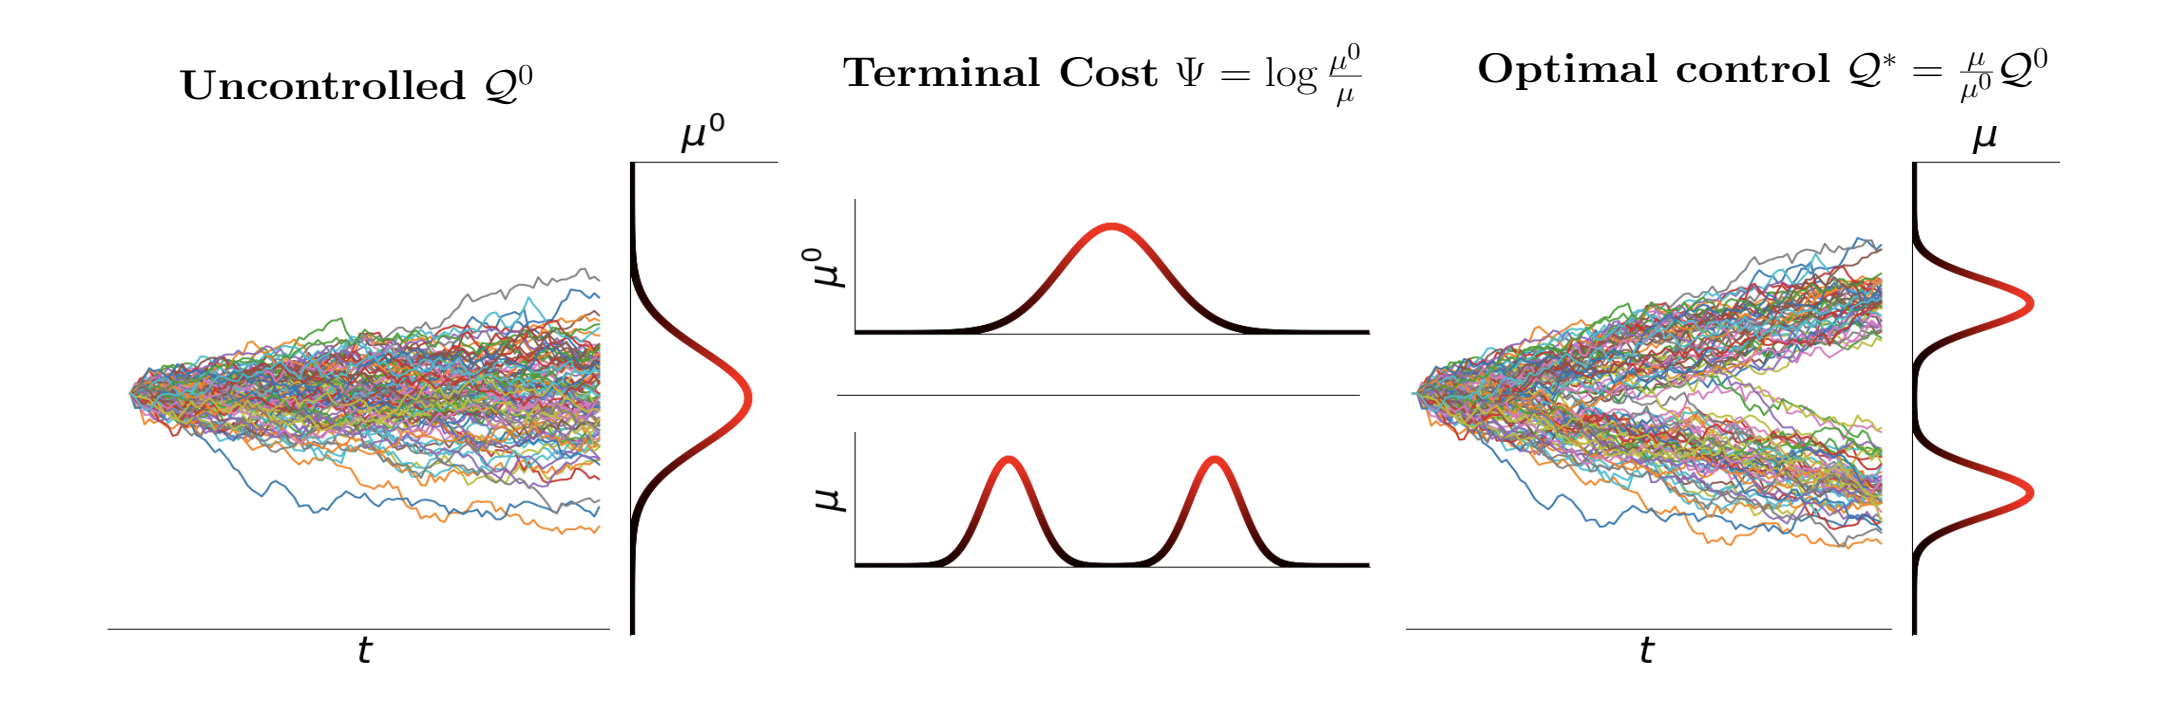
\includegraphics[width=0.6\textwidth]{figures/unconctrolled.png}
    \caption{Controlled diffusion process from simple $\nu$ to complex $\pi$.}
\end{figure}


\end{frame}

\begin{frame}[t]{SOC formulation}
\scriptsize
\textbf{SOC objective.} Choose a control $u$ to minimize
\[
\mathbb E_{Q^u}\!\left[\int_0^T \frac{1}{2\sigma^2}\|u(x_t,t)\|^2\,dt \;+\; \Psi(x_T)\right].
\]

\textbf{Pick the terminal cost to encode the target.}
\[
\Psi(x_T)\;=\;\log\frac{p_T^{\text{ref}}(x_T)}{\mu(x_T)}\quad
\big(\text{equivalently }-\log\mu(x_T)\ \text{up to } \log p_T^{\text{ref}}\big).
\]

\textbf{Key theorem (path--KL $\Leftrightarrow$ SOC).}
Define the \emph{target path measure} by terminal reweighting:
\[
P(x_{0:T})\ \propto\ Q^{\text{ref}}(x_{0:T})\ \frac{\mu(x_T)}{p_T^{\text{ref}}(x_T)}.
\]
Then, under standard regularity,
\[
\boxed{\;
D_{\mathrm{KL}}(Q^u\|P)
=\mathbb E_{Q^u}\!\Big[\int_0^T \tfrac{1}{2\sigma^2}\|u\|^2\,dt+\log\tfrac{p_T^{\text{ref}}(x_T)}{\mu(x_T)}\Big]\;+\;\text{const}
\;}
\]

\end{frame}


% --- Slide 1 ---
\begin{frame}[t]{Steps 1--2: Build forward \& reference diffusions}
\footnotesize
\textbf{Step 1 (controlled forward process).} Parameterize a sampler as a controlled diffusion:
\[
dx_t = f(x_t,t)\,dt + \sigma\,dW_t,\qquad x_0 \sim p^{\text{ref}}_0,
\]
with drift $f(\cdot,\cdot)$ (the control) to be learned. Let $Q$ denote the path law of this process.

\medskip
\textbf{Step 2 (uncontrolled reference).} Use the same noise but zero drift:
\[
dx_t = \sigma\,dW_t,\qquad x_0 \sim p^{\text{ref}}_0,
\]
whose marginals $p^{\text{ref}}_t$ are known in closed form. Let $Q^{\text{ref}}$ be its path law.

\medskip
\textbf{Goal.} Choose $f$ so that the terminal marginal of $Q$ matches the target $\pi(x)=\mu(x)/Z$ (no data, $Z$ unknown).
\end{frame}

% --- Slide 2 ---
\begin{frame}[t]{Step 3: Target path measure via terminal reweighting}
\footnotesize
\textbf{Construct a target measure on paths} by reweighting only the terminal state:
\[
P(x_{0:T}) \ \propto\ Q^{\text{ref}}(x_{0:T})\ \frac{\mu(x_T)}{p^{\text{ref}}_T(x_T)}.
\]

\textbf{Key property (endpoint correctness).}
By construction, the terminal marginal of $P$ satisfies
\[
P(x_T) \ \propto\ \mu(x_T)\quad \Longrightarrow \quad P(x_T) = \pi(x_T)\ \text{up to the (unknown) normalizer } Z.
\]

\textbf{Takeaway.} We have a principled path-space target $P$ whose endpoint is exactly the desired distribution, without ever using $Z$ along the way.
\end{frame}

% --- Slide 3 ---
\begin{frame}[t]{Step 4: Path--KL equals an SOC objective}
\footnotesize
\textbf{Match the target on path space} by minimizing a KL divergence:
\[
\min_{f}\ D_{\mathrm{KL}}\!\big(Q\ \|\ P\big).
\]

\textbf{KL--control identity (Girsanov + chain rule).}
Under standard regularity,
\[
\boxed{\
D_{\mathrm{KL}}(Q\|P)
=\ \mathbb E_{Q}\!\Big[\int_0^T \tfrac{1}{2\sigma^2}\|f(x_t,t)\|^2\,dt
\ +\ \log\tfrac{p^{\text{ref}}_T(x_T)}{\mu(x_T)}\Big]\ +\ \text{const}
}
\]

\textbf{Interpretation (SOC).}
\begin{itemize}\itemsep2pt
  \item \emph{Running cost:} $\tfrac{1}{2\sigma^2}\|f\|^2$ (control effort).
  \item \emph{Terminal cost:} $\log p^{\text{ref}}_T(x_T)-\log\mu(x_T)$ (rewards high-$\mu$ endpoints).
  \item The additive constant absorbs $+\log Z$ $\Rightarrow$ \textbf{$Z$ cancels}.
\end{itemize}

\textbf{Therefore:} Minimizing $D_{\mathrm{KL}}(Q\|P)$ is \emph{equivalent} to solving a stochastic optimal control problem.
\end{frame}

% --- Slide 4 ---
\begin{frame}[t]{Step 5 \& intuition: why this works, what remains hard}
\footnotesize
\textbf{Continuous-time view (optional).}
With $T$ fixed and finer discretization, the discrete sum becomes
\[
\min_f\ \mathbb E_Q\!\Big[\int_0^T \tfrac{1}{2\sigma^2}\|f(x_t,t)\|^2\,dt\ +\ \log\tfrac{p^{\text{ref}}_T(x_T)}{\mu(x_T)}\Big],
\]
the classic entropy-regularized SOC form.

\medskip
\textbf{Intuition (why it works).}
\begin{itemize}\itemsep2pt
  \item We \emph{steer} a simple diffusion toward regions where $\mu$ is large, trading control effort vs.\ terminal reward.
  \item The endpoint of the ideal optimizer matches $\pi=\mu/Z$ (calibrated sampling), while never needing $Z$ explicitly.
  \item Training only requires evaluating $\mu(x_T)$ (and optionally $\nabla\log\mu$), not intermediate-time scores.
\end{itemize}

\textbf{What remains hard (motivation for DGFS).}
\begin{itemize}\itemsep2pt
  \item The loss provides signal \emph{only at terminal time} $\Rightarrow$ poor credit assignment, high-variance gradients.
\end{itemize}
\end{frame}


\begin{frame}[t]{Diffusion Process}
\scriptsize

\textbf{Idea.} Let the target “diffuse to Gaussian” via a reference process (VP/VE SDE). The \emph{reverse-time} dynamics can, in principle, generate target samples if we know the \emph{score} $\nabla_x \log p_t(x)$:
\[
\underbrace{dx_t=\sigma\,dW_t}_{\text{forward/noising}}
\quad\Longleftrightarrow\quad
\underbrace{dx_t=\big[f_{\text{ref}}(x,t)-\sigma^2\nabla_x \log p_t(x)\big]dt+\sigma\,d\bar W_t}_{\text{reverse/generative}}.
\]

\textbf{What is score matching?} 
Learn a network $s_\theta(x,t)\approx \nabla_x\log p_t(x)$ by regressing on \emph{noised data}:
\[
\min_\theta\ \mathbb E_{t}\,\mathbb E_{x_0\sim p_{\text{data}}}\,\mathbb E_{\varepsilon}\!
\big\|s_\theta(x_t,t)-\nabla_x\log p_t(x_t)\big\|^2,
\]
which is equivalent to denoising a corrupted sample $x_t$ back toward $x_0$.

\vspace{0.1cm}
\begin{errorblock}{Why Denoising Score Matching is \emph{not} applicable here}
\begin{itemize}\itemsep2pt
  \item We have \emph{no dataset} from $\pi$, only the unnormalized $\mu(x)$ (and maybe $\nabla\log\mu$).

\end{itemize}
\end{errorblock}

\end{frame}

\begin{frame}[t]{Alternative to DSM: learn the vector field (control)}
\scriptsize
\textbf{Reverse SDE drift (generative side).}
\[
dx_t=\big[f_{\text{ref}}(x,t)-\sigma^2\,\nabla_x \log p_t(x)\big]\,dt+\sigma\,d\bar W_t.
\]

\textbf{DSM route (data world).} Learn the \emph{score} $s_\theta(x,t)\approx\nabla_x\log p_t(x)$ from noised \emph{data}, then plug it into the reverse drift.

\textbf{Vector-field route (our setting).} Directly learn the \emph{control/drift} $u_\theta(x,t)$ instead of the score. The two are \emph{equivalent} via:
\[
u_\theta(x,t)\;=\;f_{\text{ref}}(x,t)\;-\;\sigma^2\,s_\theta(x,t)
\quad\Longleftrightarrow\quad
s_\theta(x,t)\;=\;\tfrac{f_{\text{ref}}(x,t)-u_\theta(x,t)}{\sigma^2}.
\]

\textbf{Why do this here?}
\begin{itemize}\itemsep2pt
  \item We have no dataset from $\pi$, so DSM can’t form expectations over $p_t$; scores $\nabla\log p_t$ are unavailable.
  \item Instead, treat $u_\theta$ as a \emph{control} and \emph{learn it} by minimizing a $Z$-free \textit{path-space} KL that uses only the given $\mu(\cdot)$.
  \item This sets up diffusion samplers à la PIS/DDS and enables DGFS’s improvements (intermediate, subtrajectory credit).
\end{itemize}

\textbf{Notation tip.} Use $u_\theta$ (or $f$) for the vector field to avoid clashing with $\mu(\cdot)$, which denotes the unnormalized density.
\end{frame}

% \begin{frame}{Diffusion Sampler}

% \end{frame}


\begin{frame}[t]{Sampling as a Stochastic Optimal Control problem}
\footnotesize
\textbf{Forward (controlled) process $Q$.} A Markov chain with Gaussian transitions:
\[
Q(x_{0:N}):\quad x_0\sim p_0^{\text{ref}},\quad x_{n+1}\sim P_F(\cdot\mid x_n)=\mathcal N\!\big(x_n + h\,f(x_n,n),\; h\sigma^2 I\big).
\]

\textbf{Reference process $Q^{\text{ref}}$.} Same covariance, zero drift:
\[
x_{n+1}\sim P_F^{\text{ref}}(\cdot\mid x_n)=\mathcal N\!\big(x_n,\; h\sigma^2 I\big),\qquad x_0\sim p_0^{\text{ref}},\ \ p_n^{\text{ref}}\text{ known.}
\]

\textbf{Target process $P$.} Tie the terminal marginal to $\pi$ via the reference:
\[
P(x_{0:N})\ :=\ Q^{\text{ref}}(x_{0:N})\;\frac{\pi(x_N)}{p_N^{\text{ref}}(x_N)}.
\]
Then $P(x_N)\propto \mu(x_N)$, making $P$ a valid path-space target.
\end{frame}

\begin{frame}[t]{Sampling as a Stochastic Optimal Control problem}
\footnotesize

\medskip
\textbf{Learning objective (discrete-time SOC).} Learn $f$ by minimizing the path KL:
\[
\min_{f}\ D_{\mathrm{KL}}(Q\ \|\ P)
\;\;\Longleftrightarrow\;\;
\min_{f}\ \mathbb E_{Q}\!\Big[\sum_{n=0}^{N-1}\frac{h}{2\sigma^2}\,\|f(x_n,n)\|^2\;+\;\log\Psi(x_N)\Big],
\]
with \(\Psi(x_N)=\dfrac{p_N^{\text{ref}}(x_N)}{\mu(x_N)}\).
(Continuous-time limit recovers the classic VE-SDE SOC formulation.)
\end{frame}

\begin{frame}[t]{Why SOC, and what still hurts (motivation for DGFS)}
\footnotesize
\textbf{Why SOC/control-as-inference?}
\begin{itemize}\itemsep3pt
  \item Principled \emph{path-space} objective; $Z$ cancels, so only $\mu$ (and optionally $\nabla\log\mu$) is needed.
  \item Calibrated sampling by \emph{steering} a simple reference process toward the target.
\end{itemize}

\textbf{Pain point in prior SOC samplers (PIS/DDS).}
\begin{itemize}\itemsep3pt
  \item Training signal sits \emph{only at terminal time} $N$ and losses use \emph{full trajectories} $\Rightarrow$ poor credit assignment, high variance, weaker mode coverage.
\end{itemize}

\textbf{DGFS in one line.}
\begin{itemize}\itemsep3pt
  \item Keep the same SOC/path-KL setup, but introduce a learned \emph{flow function} $F_n(x_n)$ and enforce \emph{subtrajectory balance} to inject \emph{intermediate} learning signals and enable \emph{partial-trajectory} training.
\end{itemize}
\end{frame}



\subsection{Limitations of Prior Work}




%------------------------------------------------
\section{Methodology}

\subsection{DGFS framework}


%------------------------------------------------
\section{Results and Limitations}

\subsection{Results}


%------------------------------------------------
\section{Conclusion}

\subsection{Key Insights}
% Add content: Summarize DGFS's impact and paper's contributions.

\subsection{Future Directions and Usage since its release}
% Add content: Discuss limitations, extensions, and personal thoughts.

\begin{frame}{Conclusion}

\end{frame}


\end{document}